\documentclass[
    % -- opções da classe memoir --
    article,			% indica que é um artigo acadêmico
    12pt,				% tamanho da fonte
    oneside,            % o texto vá ser impresso em apenas um lado, alinhamento igual nas páginas. Oposto do twoside
    a4paper,			% tamanho do papel.
    english,			% idioma adicional para hifenização
    brazil,				% o último idioma é o principal do documento
    ]{abntex2}

%--------------------------------------------------------------------
%                              PACOTES 
%--------------------------------------------------------------------

%---
% Pacotes Fundamentais 
%---
\usepackage{sbc-template}           % usa o modelo sbc
\usepackage{times}                  % usa a fonte Times new Roman
\usepackage[T1]{fontenc}            % seleção de codigos de fonte.
\usepackage[utf8]{inputenc}         % conversão automática dos acentos
\usepackage{indentfirst}            % indenta o primeiro parágrafo de cada seção.
\usepackage{nomencl}                % lista de simbolos
\usepackage{color}	                % controle das cores
\usepackage{graphicx}               % gerenciar imagens 
\usepackage{microtype}              % para melhorias de justificação


%---
% Pacotes adicionais
%---
\usepackage{ragged2e}              % insere o alinhamento justificado ao texto.
\usepackage{setspace}              % alterar o espaçamento (padrão: simples)
    \onehalfspacing                % definindo espaçamento de 1.5
    \setlength{\parindent}{1.25cm} % tamanho do parágrafo 
\usepackage{float}                 % que disponibiliza a opção [h] para fixar a imagem  
\usepackage{url}                   % definir opções para a url

%definir as dimensões das páginas
\usepackage[lmargin=3cm, tmargin=3cm, rmargin=2cm, bmargin=2cm]{geometry}  


% ---
% Pacotes de citações
% ---
\usepackage[brazilian,hyperpageref]{backref}	 % paginas com as citações na bibl
\usepackage[alf]{abntex2cite}	                 % citações padrão ABNT
\sloppy                                          % com esse comando tem menor possibilidade de incidência das linhas muito extensas (ainda mais url) 


%--------------------------------------------------------------------
%                        Configurações 
%--------------------------------------------------------------------

% alterando o aspecto da cor azul
\definecolor{blue}{RGB}{41,5,195}


% informações do PDF
\makeatletter                                           
\hypersetup{
        %pagebackref=true,
		pdftitle={\@title}, 
		pdfauthor={\@author},
    	pdfsubject={\imprimirpreambulo},
	    pdfcreator={LaTeX with abnTeX2},
		pdfkeywords={abnt}{latex}{abntex}{abntex2}{trabalho acadêmico}, 
		colorlinks=true,     % false: links em caixa; verdadeiro: links coloridos
    	linkcolor=blue,      % cor dos links internos
    	citecolor=blue,      % cor dos links para bibliografia
    	filecolor=magenta,   % cor dos links do arquivo
		urlcolor=blue,
		bookmarksdepth=4
}
\makeatother

% Define os textos da citação
\renewcommand*{\backrefalt}[4]{
	\ifcase #1 %
		Nenhuma citação no texto.%
	\or
		Citado na página #2.%
	\else
		Citado #1 vezes nas páginas #2.%
	\fi}%
% ---

%%%%%%%%%%%%%%%%%%%%%%%%%%%%%%%%%%%%%%%%%%%%%%%%%%%%%%%%%%%%%%%%%%%%
%                           Início 
%%%%%%%%%%%%%%%%%%%%%%%%%%%%%%%%%%%%%%%%%%%%%%%%%%%%%%%%%%%%%%%%%%%%

\title{Voz Feminina}

\author{Izadora Martins da Silva, Kauanne Paula de Oliveira, Laís Higuti Leite, \\ Lie Higuti Leite, Matheus Augusto Preto Santana}

\address{Instituto Federal de Educação, Ciência e Tecnologia de São Paulo (IFSP)\\ São Paulo -- SP -- Brasil \\ Curso Técnico em Informática Integrado ao Ensino Médio
\nextinstitute
  PDS - Prática para Desenvolvimento de Sistemas
  \email{\{izadora.martins,k.paula,lais.higuti,lie.higuti,m.preto\}@aluno.ifsp.edu.br}\\\\
}

\begin{document} 

\maketitle

\begin{abstract}
    The document addresses violence against women in Brazil from the colonial era to the present, highlighting the persistence of patriarchal culture and gender inequalities. Despite the creation of laws such as the Maria da Penha Law, violence continues due to underreporting and impunity, particularly noted during the COVID-19 pandemic when domestic violence cases increased significantly. In response, the Voz Feminina app was developed to raise awareness and support victims. The document also mentions the victims' lack of trust in the justice system and emphasizes the importance of early interventions and improved support services. Additionally, it describes the technologies and methods used in software development.\end{abstract}
     
\begin{resumo1} 
    O documento trata da violência contra as mulheres no Brasil, desde a era colonial até hoje, destacando a persistência da cultura patriarcal e das desigualdades de gênero. Embora leis como a Lei Maria da Penha tenham sido criadas, a violência continua devido à subnotificação e à impunidade, como na época da pandemia da COVID-19 onde casos de violência doméstica aumentaram significativamente. Em resposta, o aplicativo Voz Feminina foi desenvolvido para conscientizar e apoiar as vítimas. O documento também menciona a falta de confiança das vítimas no sistema de justiça e a importância de intervenções precoces e de melhores serviços de apoio. Além disso, descreve as tecnologias e métodos utilizados no desenvolvimento de software.
\end{resumo1}

\section{Introdução}
\pagestyle{plain}
\pagenumbering{arabic}
    A violência contra as mulheres no Brasil é uma realidade antiga, cujas raízes mergulham profundamente na história do país. Na era colonial, quando a estrutura patriarcal foi estabelecida com a chegada dos portugueses, ocorreram diversas práticas exploratórias e violentas, especialmente contra mulheres negras e indígenas, que eram submetidas a abusos sexuais e violência física. Já no período imperial, quando foi estabelecida a independência do Brasil, a violência de gênero era evidente, com mulheres brancas sendo submetidas a um papel de submissão e recato, enquanto os homens tinham liberdade no espaço público. Mulheres negras eram alvo de abusos sexuais e violência por parte das esposas dos senhores, replicando a violência que elas mesmas sofriam. Além disso, muitas escravas eram prostituídas e exploradas como amas de leite, sendo obrigadas a amamentar os filhos de mulheres brancas em detrimento de seus próprios filhos. A violência de gênero e a exploração sexual eram práticas comuns nesses períodos históricos, que refletiam a estrutura patriarcal, escravocrata do país e a forma de manter a ordem social estabelecida \cite{colonialImpep_2019}.

    Após a saida do Brasil da monarquia, surgiu a República Velha (1889-1930) onde as estruturas de poder persistiram, alimentadas por noções arraigadas de masculinidade e feminilidade. A ideia de inferioridade das mulheres em relação aos homens, e consequentemente na justificação de tratamento desigual, permeava todos os aspectos da vida social e jurídica. Isso não apenas perpetuava a violência contra as mulheres, mas também as submetia a uma série de desafios decorrentes das estruturas patriarcais e normas sociais da época. Elas eram politicamente excluídas, não tinham direito ao voto nem podiam candidatar-se a cargos políticos, limitando sua participação política e social. Na educação, o acesso era restrito, com foco em papéis domésticos, enquanto socialmente eram pressionadas a serem esposas e mães submissas. A violência contra as mulheres era tolerada e invisibilizada, com poucos recursos para as vítimas e apesar das resistências, como os movimentos sufragistas, a participação política feminina era mínima. A República Velha representou um período de desigualdade de gênero, com as mulheres enfrentando obstáculos que limitavam suas oportunidades e autonomia \cite{repvelha_2018}.

    A ditadura militar (1964-1985) foi um período sombrio não só politicamente, mas também para os direitos das mulheres. A violência específica contra mulheres militantes evidenciava relações de poder assimétricas, como a violência de gênero que é fundamental para entender ações violentas em contextos sociais, destacando as desigualdades de gênero. A cultura patriarcal brasileira é o elemento central na manutenção de hierarquias de gênero e construção de papéis sociais \cite{ditadura_2019}. 
    
    No relatório da Comissão Nacional da Verdade (CNV) é abordado a violência sexual e física sofrida por mulheres, incluindo tortura sexual como choques elétricos nas genitais, porém não se limitou apenas a ataques sexuais, abrangendo também violência verbal, ameaças e humilhações. Essas práticas sistemáticas do Estado, visava silenciar mulheres que desafiavam estereótipos de gênero e que lutavam por participação política. Durante esse período, a violência de gênero contra mulheres atingiu níveis extremos, refletindo relação entre autoritarismo e representações patriarcais, usada como instrumento de dominação masculina e para manter desigualdades entre os sexos \cite{ditaduraBR_2020}.

    Com o fim da ditadura em 1985, surgiu um novo período chamado "República Nova", onde a violência contra a mulher teve cada vez mais reconhecimento como um direito humano e de justiça social. O aumento da conscientização pública sobre a violência contra a mulher foi impulsionado principalmente por movimentos sociais, campanhas de sensibilização e a atuação de organizações da sociedade. Isso resultou em um maior reconhecimento do problema e na criação de serviços de apoio às vítimas, como centros de acolhimento, delegacias especializadas e redes de assistência jurídica \cite{15anosLMP_2022} \cite{LMPavanços_2016}.
    
    Além disso, diversas leis foram promulgadas para proteger as mulheres contra a violência doméstica e garantir a igualdade de gênero em diferentes esferas da sociedade. A lei que posssue um maior reconhecimento é a Lei Nº 11.340/2006, Lei Maria da Penha, que foi criada para reprimir e prevenir a violência doméstica e familiar contra as mulheres. Ela recebeu esse nome em homenagem a mulher Maria da Penha Maia Fernandes, que foi vítima de violência doméstica e lutou por anos para ver seu agressor responsabilizado. No entanto, para que implementação efetiva dessas leis e políticas acontecesse, houve uma série de obstáculos devido à resistência cultural, falta de recursos e capacitação inadequada das instituições responsáveis pela aplicação das leis \cite{15anosLMP_2022} \cite{LMPavanços_2016}.

    De modo igual, a cultura popular e os meios de comunicação social desempenham um papel significativo na perpetuação da violência baseada no gênero, principalmente através dos estereótipos que retratam as mulheres como objetos sexuais, figuras submissas e com uma beleza impecável. Na mídia, essas representações acabam normalizando a violência e dificultando o enfrentamento dessa realidade. A dominação masculina nesse meio promove ativamente o mito da beleza, reduzindo a mulher à sua aparência e perpetuando diversas formas de violência, seja física, psicológica ou social. Na construção dessas representações, é comum a imprensa retratar estereótipos que desrespeitam os direitos das mulheres utilizando imagens femininas não apenas para promover produtos, mas também para incitar o consumo, fortalecendo ainda mais a dominação masculina. Essas representações equivocadas afetam profundamente a identidade feminina, perpetuando assim a violência de gênero \cite{mulhermidia_2018}.

    No entanto, apesar dos esforços para enfrentar a violência de gênero, os índices continuam alarmantes. A violência doméstica, o feminicídio, o assédio sexual e outras formas de violência contra a mulher ainda são uma realidade cotidiana para muitas brasileiras. Além disso, a subnotificação e a impunidade persistem como desafios significativos para a erradicação desse problema.

\subsection{Objetivo}

    O aplicativo Voz Feminina procura conscientizar e fornecer suporte para que as mulheres possam denunciar ou discutir as violências que enfrentam ou enfrentaram, indo além da violência doméstica e familiar descrita na Lei Maria da Penha, abrangendo também assédios sexuais e morais no ambiente de trabalho e na rua. Buscamos criar uma rede de apoio onde as mulheres sintam-se confortáveis para compartilhar suas histórias e aconselhar outras que possam estar passando por experiências similares.

\subsection{Justificativa}

    A décima edição da Pesquisa Nacional de Violência contra a Mulher, conduzida pelo Instituto DataSenado em parceria com o Observatório da Mulher contra a Violência (OMV) e divulgada em 2023, trouxe à tona novos dados sobre a realidade da violência enfrentada pelas mulheres brasileiras. De acordo com o gráfico, representado na figura 1, destaca-se que 48\% das cidadãs de São Paulo consideram que as mulheres não são tratadas com o devido respeito no Brasil, evidenciando uma preocupante percepção sobre a igualdade de gênero na sociedade. Além disso, é importante ressaltar que a preocupação com a desigualdade de gênero não se restringe apenas às mulheres de São Paulo, mas reflete uma percepção nacional. A pesquisa revelou que, em todo o Brasil, a porcentagem de mulheres que consideram que as mulheres não são tratadas com o devido respeito foi de 46\%, enquanto apenas 7\% afirmaram que as mulheres são tratadas com respeito. Esses números demonstram que a questão da igualdade de gênero é uma preocupação generalizada em todo o país, exigindo ações concretas para promover mudanças significativas nesse cenário \cite{senadoBR_2021} \cite{senadoSP_2023}.

\begin{figure}[ht]
    \centering
    \includegraphics[width=11cm]{são tratadas com respeito.png}\\
    \caption{“De forma geral, você acha que as mulheres são tratadas com respeito no Brasil?”}
        Fonte: Adaptado da 10° edição da Pesquisa Nacional de Violência contra a Mulher
    \label{fig:infografico}
\end{figure}

    Não é mera coincidência que a maioria das mulheres tenha respondido "Não" \space quando questionadas se as mulheres são tratadas com respeito. Isso reflete a persistência de um sistema social e cultural que concede poder e privilégios aos homens, permitindo que desrespeitem mulheres em diferentes contextos, como na rua, no trabalho e em casa. Essas relações desiguais de gênero e poder exacerbam a violência contra a mulher, perpetuando-a como algo normalizado. Essa violência não se limita apenas ao âmbito físico, mas também se manifesta por meio de normas sociais, expectativas culturais e práticas discriminatórias que reforçam a dominação masculina. 

    Na mesma pesquisa feita pelo Instituto DataSenado, as mulheres apontaram que o ambiente que sentem menos respeitadas é principalmente na rua (53\%), seguido pelo ambiente de trabalho (24\%) e dentro da própria família (17\%). É apresentado resultados onde 30\% das mulheres entrevistadas, em São Paulo, declararam terem sido vítimas de violência doméstica ou familiar provocada principalmente por homens, com 20\% desses casos ocorrendo nos últimos 12 meses (figura 2). A violência psicológica foi identificada como a forma mais recorrente de agressão, relatada por 90\% das mulheres que sofreram violência doméstica ou familiar, seguida pelas violências física (77\%) e moral (76\%) \cite{senadoSP_2023}.

\begin{figure}[ht]
    \centering
    \includegraphics[width=12cm]{epsodio e já sofreu.png}\\
    \caption{“Pesquisa sobre episódios de violência doméstica”}
        Fonte: Adaptado da 10° edição da Pesquisa Nacional de Violência contra a Mulher
    \label{fig:infografico}
\end{figure}

    Durante a pandemia de COVID-19, a violência contra a mulher no Brasil se intensificou. Relatórios da OMS e da OPAS destacam a violência contra as mulheres como um problema grave, agravado pela crise sanitária. Dados da Conferência Nacional dos Municípios (CNM) mostram que 20\% dos 2.383 municípios pesquisados relataram aumento da violência doméstica, e as denúncias chegaram a 105.821 em 2020 \cite{relatorio}.

    O período de quarentena foi particularmente crítico. Em São Paulo, a Prefeitura atendeu 24.113 mulheres em 12 equipamentos de proteção, com uma queda acentuada nos atendimentos entre abril e maio, seguida por uma recuperação gradual, alcançando um pico de 2.890 casos em novembro. A Secretaria Municipal de Direitos Humanos e Cidadania reforçou o suporte às vítimas, com 13 serviços funcionando e atendimento especializado \cite{cidadeSP_2021} \cite{vulnerabilidadeCovid_2020}.

    Embora tenha havido uma leve redução na quantidade de mulheres agredidas em comparação com 2017 e 2019, a natureza da violência mudou. O percentual de mulheres agredidas caiu de 27,4\% em 2019 para 24,4\% em 2021 e a violência nas ruas diminuiu de 39\% para 19\%, enquanto a violência doméstica aumentou de 43\% para 49\%. A maioria dos agressores são parceiros íntimos ou ex-parceiros, e a violência por familiares também se tornou mais evidente \cite{pandemia}.

    Com esse aumento da violência doméstica, ouve uma necessidade de implementar ações de suporte para mulheres, que intencificou a preocupação com a segurança e o bem-estar das mulheres em seus lares. A análise feita pelo DataSenado releva uma questão alarmante, refletida no expressivo percentual de 69\% das mulheres que acreditam que a violência doméstica aumentou nos últimos doze anos, apresentado no gráfico da figura 3 \cite{senadoSP_2023}. Esse dado ressalta uma tendência preocupante e indica uma deterioração das condições de segurança para as mulheres dentro de suas próprias residências ao longo do tempo. O aumento da percepção de risco pode ser atribuído a uma série de fatores, incluindo mudanças nas dinâmicas familiares, pressões socioeconômicas e até mesmo um maior reconhecimento e conscientização sobre o problema da violência doméstica. Independentemente das causas subjacentes, é evidente que a violência doméstica continua a ser uma ameaça séria e crescente para as mulheres, exigindo respostas eficazes por parte da sociedade e das autoridades para garantir a proteção e a segurança de todas as mulheres em seus lares. 

\begin{figure}[ht]
    \centering
    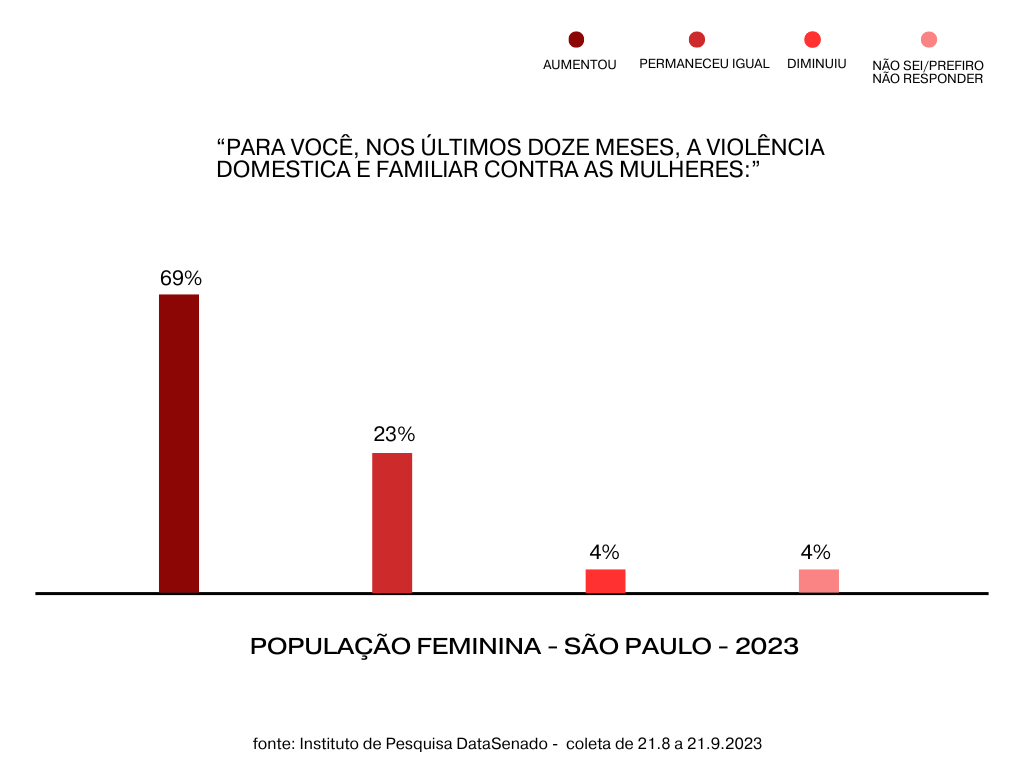
\includegraphics[width=12cm]{violencencia domestica e familiar.png}\\
    \caption{“Aumento da violência doméstica contra as mulheres”}
        Fonte: Adaptado da 10° edição da Pesquisa Nacional de Violência contra a Mulher
    \label{fig:infografico}
\end{figure}

    A maioria dos casos de violência doméstica tende a ocorrer durante a juventude da mulher devido a uma série de fatores complexos profundamente preocupante, pois sugere que a violência de gênero está enraizada desde cedo na vida das vítimas. Segundo o IBGE, cerca de 9,2\% das mulheres que relataram ter sofrido uma violência, tinha idade entre 18 e 19 anos, dados muitos parecidos com a pesquisa feita pelo DataSenada, onde 36\% tiveram a primeira agressão em torno dessa faixa etária \cite{IBGE} \cite{senadoSP_2023}. Isso ressalta a urgência de intervenções precoces e eficazes para prevenir a perpetuação desse ciclo de violência ao longo da vida das mulheres. Essa constatação também lança luz sobre a importância da educação e conscientização desde a juventude para promover relacionamentos saudáveis e respeitosos.

    Uma pesquisa realizada pelo Instituto de Pesquisas Sociais, Políticas e Econômicas (Ipespe) entre 21 e 24 de agosto de 2021, revelou que 73\% das mulheres não denunciam a violência devido ao medo e 31\% por vergonha \cite{violenciaemdados}. O mesmo estudo destacou que as formas mais comuns de violência são ofensas verbais (18,6\%), ameaças físicas (8,5\%), ofensas sexuais (5,4\%), ameaças com armas (3,1\%) e espancamento ou tentativa de estrangulamento (2,4\%). Preocupantemente, 44,9\% das mulheres não tomaram nenhuma atitude em relação à agressão mais grave, e apenas 11,8\% procuraram ajuda nas delegacias da mulher \cite{relatorio}.

    A pesquisa feito pelo DataSenado, revelou que 16\% das mulheres foram psicologicamente intimidada por seus agressores, um indicador de como muitos comportamentos abusivos são ignorados ou minimizados  \cite{senadoSP_2023}. Isso sublinha a necessidade de uma educação mais ampla sobre as diferentes formas de violência de gênero para que as vítimas possam reconhecer e reagir adequadamente. O medo das retaliações do agressor é um grande obstáculo para a denúncia, refletindo a opressão psicológica que as vítimas enfrentam. Muitas vezes, esse medo é justificado pela experiência de que denunciar pode trazer consequências tão graves quanto o próprio abuso, exacerbado pela ineficácia das autoridades em proteger as vítimas e punir os agressores.

    Além disso, 62\% das mulheres não denunciam devido à dependência financeira, que as mantém presas em relações abusivas e dá aos agressores um controle adicional sobre suas vidas. A falta de recursos é muitas vezes agravada por uma cultura que culpa as vítimas e minimiza a gravidade da violência doméstica. Também, a crença de que a violência será a última vez que ocorre contribui para a hesitação em buscar ajuda, destacando a complexidade emocional das situações de abuso e a esperança muitas vezes frustrada de que o agressor mudará \cite{senadoSP_2023}.

    A impunidade percebida e o medo do agressor são desafios significativos que impedem as mulheres de denunciar casos de violência. A cultura do silêncio, combinada com a falta de apoio adequado e a precariedade dos serviços públicos, torna ainda mais difícil para as vítimas buscar ajuda e proteção, perpetuando assim o ciclo de violência. Referente a Pesquisa Nacional de Violência contra a Mulher, ilustrada na figura 4, 65\% das mulheres admitiram não ter buscado qualquer tipo de assistência de saúde devido à violência que enfrentavam, enquanto apenas 34\% afirmaram ter procurado. Esse cenário evidencia as barreiras significativas que as mulheres enfrentam ao tentar acessar serviços de saúde em contextos de violência. Além disso, ressalta a importância de abordagens proativas na identificação e no apoio às vítimas dentro dos serviços de saúde, garantindo que elas se sintam seguras e apoiadas ao buscar assistência, e que recebam o suporte necessário para romper o ciclo de violência e recuperar sua saúde física e emocional \cite{saude_2009}.

 \begin{figure}[ht]
    \centering
    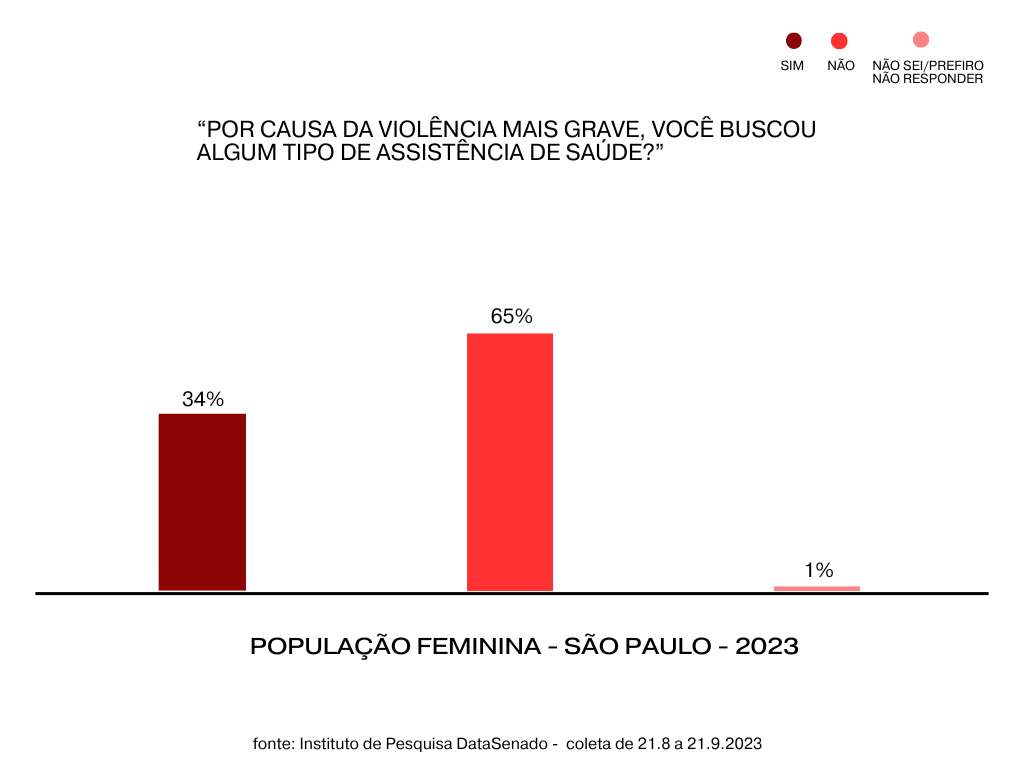
\includegraphics[width=11cm]{buscou assistencia de saude.png}\\
    \caption{“Pesquisa sobre buscar a assistência de saúde”}
        Fonte: Adaptado da 10° edição da Pesquisa Nacional de Violência contra a Mulher
    \label{fig:infografico}
\end{figure}

    A análise das denúncias de agressões revela uma profunda desconfiança no sistema de justiça e segurança pública por parte das vítimas. Apenas 1\% das mulheres acreditam que as denúncias são sempre feitas às autoridades, o que sugere uma falta de confiança fundamentada em experiências anteriores de não serem levadas a sério ou de enfrentarem revitimização durante o processo de denúncia \cite{senadoSP_2023}.

    Por outro lado, um estudo feito pelo Mapa Nacional da Violência de Gênero apresenta um aumento entre as mulheres em procurar ajuda por meio da família (60\%), da religião (42\%), amigos (40\%) e denunciar em delegacias (31\%); além da maioria das mulheres entrevistadas pelo Observatório da mulher (67\%) também acreditarem que, na maioria das vezes, as mulheres acabam denunciando, reforçando uma tendência crescente de buscar ajuda e reportar os abusos sofridos \cite{senadoSP_2023}. Isso pode refletir uma maior conscientização sobre a importância da denúncia e um fortalecimento das redes de apoio disponíveis, além do acesso ampliado a informações sobre os direitos das mulheres. 

    No entanto, a discrepância entre a percepção das mulheres sobre a frequência das denúncias e os números reais de casos registrados pelas autoridades sugere uma possível subnotificação e falta de visibilidade dos casos de violência contra a mulher. Isso ressalta a necessidade imediata de aprimorar os mecanismos de denúncia e garantir um ambiente seguro e solidário para as vítimas, visando aumentar a confiança e a disposição para reportar esses casos.

    Adicionalmente, a pesquisa também aponta os motivos pelos quais muitas mulheres optam por não denunciar. A sensação de impunidade, percebida por cerca de 62\% das entrevistadas, e o medo do agressor, relatado por 73\%, são fatores significativos que contribuem para o subregistro desses casos. Esse cenário é ainda mais alarmante diante do aumento de 22\% nos casos de violência contra a mulher em 2023 em comparação ao ano anterior, evidenciando a gravidade e a persistência desse problema \cite{senadoSP_2023}.

    A Lei Maria da Penha, promulgada em 2006, é amplamente reconhecida e respeitada por sua contribuição significativa na luta contra a violência doméstica. Dados mostram que a lei ajudou a reduzir em cerca de 10\% os homicídios de mulheres em suas residências. A Lei Maria da Penha é conhecida por 98\% dos brasileiros, e 86\% acreditam que ela incentivou um aumento nas denúncias de violência doméstica \cite{lei-covid}.

    Apesar desses avanços, a eficácia da Lei Maria da Penha enfrenta desafios significativos. A percepção de sua eficácia entre as mulheres é preocupante, referente a figura 5, apenas 23\% considerando a lei eficaz. Esse sentimento de desconfiança revela falhas potenciais na aplicação da lei e na resposta das autoridades às denúncias de violência. Além disso, 22\% das mulheres não acreditam que a lei é suficiente para lidar com a complexidade da violência doméstica, o que destaca a necessidade de fortalecer as medidas de proteção e promover uma cultura de responsabilização \cite{senadoSP_2023}.

\begin{figure}[ht]
    \centering

    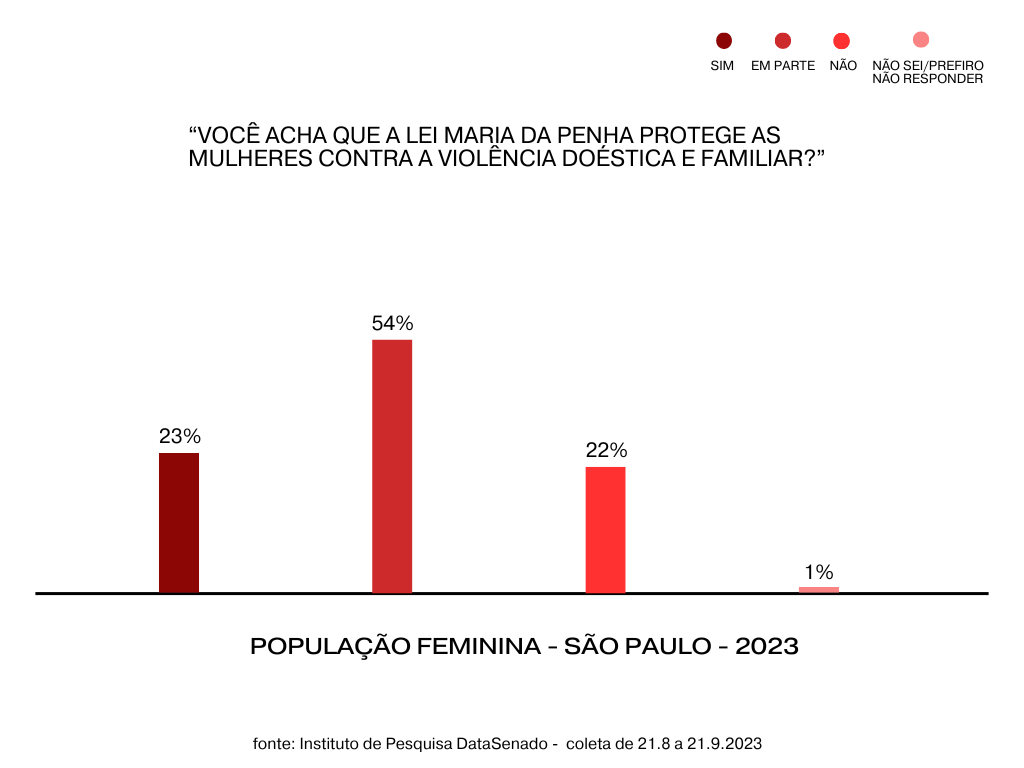
\includegraphics[width=12cm]{lei maria da penha protege.png}\\
    \caption{“Lei maria da Penha e proteção”}
        Fonte: Adaptado da 10° edição da Pesquisa Nacional de Violência contra a Mulher
    \label{fig:infografico}
\end{figure}

    Dados do DataSenado de 2019 indicam que uma em cada cinco mulheres já foi espancada por um parceiro ou ex-parceiro. Embora a maioria das brasileiras conheça a Lei Maria da Penha, muitas ainda se sentem desrespeitadas e insatisfeitas com a proteção oferecida. O contexto de pandemia agravou a situação, com um aumento nos casos de violência doméstica e uma redução nas denúncias, muitas vezes devido à proximidade com os agressores e ao medo de descumprir as medidas de isolamento social \cite{lei-covid}.

    Por conseguinte, a efetividade da Lei Maria da Penha depende não apenas da sua existência legal, mas também da sua implementação eficaz e do fortalecimento das políticas públicas que abordam as causas estruturais da violência. A interseccionalidade nesse contexto é crucial para assegurar que todas as mulheres, especialmente aquelas pertencentes a grupos vulneráveis, tenham acesso igualitário à proteção e aos serviços de apoio \cite{LMPavanços_2016}.

    As informações destacadas nos textos são de extrema importância para um aplicativo que aborda as vulnerabilidades enfrentadas pelas mulheres seja desenvolvido com eficiência. Entender os desafios específicos que as mulheres enfrentam, é essencial para desenvolver recursos e serviços adequados que possam oferecer suporte e assistência eficazes. Ao reconhecer o cárcere privado e a suspensão de serviços essenciais, o aplicativo pode direcionar seus esforços para fornecer informações e recursos relevantes sobre como as mulheres podem proteger sua segurança e buscar ajuda quando necessário.

    Além disso, ao abordar o silenciamento e a invisibilização da violência contra a mulher, o aplicativo pode promover a conscientização e a educação sobre os direitos das mulheres e aos sinais de abuso, incentivando-as a denunciar e buscar apoio. A compreensão das causas subjacentes da violência, como a falta de renda, o desemprego e a precarização dos programas de assistência, permite que o aplicativo ofereça recursos para enfrentar esses problemas de forma proativa. 
    
    Diante desse cenário, em um projeto acadêmico da disciplina de Prática de Desenvolvimento de Sistemas (PDS) do Instituto Federal de São Paulo (IFSP), a equipe KLIM decidiu abordar esse tema delicado. Composta majoritariamente por mulheres, a equipe sentiu a necessidade de agir em prol das vítimas de violência contra a mulher buscando criar uma rede de apoio onde elas possam se sentir seguras e recebam assistência para reconstruírem suas vidas após essas experiências desafiadoras.

\section{Materiais e Métodos}
     Está seção proporciona uma descrição detalhada das tecnologias que serão empregadas, bem como suas respectivas aplicações. Temos como meta oferecer uma compreensão dos recursos empregados e dos processos implementados, englobando ambientes de desenvolvimento integrado, frameworks, linguagens de programação, além de ferramentas para controle de versão, armazenamento de dados, entre outros. Adicionalmente, discorreremos sobre as práticas adotadas dos materiais, escolhidas com base nas funcionalidades que melhor se alinham com nossa situação e metas.
    
\subsection{Materiais}
    Os materiais abarcam as tecnologias utilizadas durante a produção do nosso software. O objetivo é proporcionar uma visão abrangente dos recursos tecnológicos empregados, auxiliando na compreensão das bases que sustentam o desenvolvimento da aplicação. A seguir, estão os materiais usados para a elaboração da Voz Fermina, contendo uma breve explicação e o motivo de serem escolhidos.
    
\begin{enumerate}
    \item Front-end \\
        O front-end é a parte visível para os usuários, englobando elementos como botões, caixas de seleção, gráficos e mensagens de texto. Essa interface gráfica, desenvolvida no  front-end, é o ponto de contato direto entre o usuário e o projeto.\\

\begin{description}
    \item[a)] JavaScript \par JavaScript é uma linguagem de programação interpretado e orientado a objetos. Suas funcionalidades podem aprimorar a experiência do usuário durante a navegação, desde a atualização dinâmica de feeds até a exibição de animações \cite{JS}. Foi selecionado por incorporar interatividade e dinamismo ao nosso aplicativo, levando em consideração também o amplo suporte disponível dessa linguagem. \\

    \item[b)] React Native \par React Native é um framework de desenvolvimento de aplicativos móveis multiplataforma, compatível com iOS e Android, e baseado na linguagem JavaScript. React Native permite criar aplicativos verdadeiramente nativos e não compromete a experiência dos usuários \cite{reactnative}. Será utilizado devido à sua simplicidade, praticidade e amplo suporte disponível. \\

    \item[c)] Expo Router \par O Expo Router é um sistema de roteamento baseado em arquivos, projetado para aplicações React Native e web \cite{Navegação_RN/ER}. Ele facilita o gerenciamento da navegação entre as telas do aplicativo, garantindo que os usuários possam transitar sem problemas entre diferentes partes da interface do usuário usando os mesmos componentes em diversas plataformas. A utilização será devido à facilidade de gerenciamento da navegação entre telas e para integrá-lo com o React Native. \\

    \item[d)] Bootstrap \par O Bootstrap é um framework de código aberto que disponibiliza componentes prontos para uso em projetos, permitindo criar e personalizar sites responsivos para uma variedade de dispositivos, incluindo desktops, notebooks e dispositivos móveis \cite{Bootstrap}. Será utilizado o Bootstrap devido à sua capacidade de acelerar o processo de desenvolvimento, oferecendo componentes pré-construídos e simplificando a criação de layouts responsivos. \\  
\end{description}

    \item Back-end \\
        O back-end está relacionado com os dados e a infraestrutura que garantem o funcionamento do software. Ele abriga o banco de dados e os servidores, responsáveis por armazenar e processar os dados para os usuários. Além disso, é onde são implementadas medidas de segurança, estruturação e gerenciamento de conteúdo. \\
        
\begin{description}
    \item[a)] Node.js \par O Node.js é um ambiente de execução JavaScript que permite executar aplicações desenvolvidas com a linguagem de forma autônoma, sem depender de um navegador \cite{node.js}. Será aplicado devido a flexibilidade e eficiência que essa tecnologia proporcionará a aplicação. \\
\end{description}

    \item Banco de dados \\
        O banco de dados é a organização e armazenagem de informações sobre um domínio específico. De forma mais simples, é o agrupamento de dados que tratam do mesmo assunto, e que precisam ser armazenados para segurança ou comparação futura. \\
        
\begin{description}
    \item[a)] MariaDB \par O MariaDB é um banco de dados de código aberto com um modelo de cliente-servidor. É um software utilizado para criar e gerenciar bancos de dados baseados no modelo relacional, ademais é amplamente compatível com o MySQL em vários aspectos: todos os comandos, interfaces, bibliotecas e APIs disponíveis no MySQL também estão presentes no MariaDB \cite{MariaBD}. Decidimos usufruir dele pela familiaridade com MySQL e por ser gratuito. \\
\end{description}

    \item Ambiente de Desenvolvimento Integrado \\
        Um ambiente de desenvolvimento integrado (IDE) é uma ferramenta de software para criar aplicações, que reúne diversas ferramentas de desenvolvedor em uma única interface gráfica. O IDE aumenta a produtividade do desenvolvedor ao combinar recursos como edição, compilação, teste e empacotamento de software em uma interface fácil de usar. \\
        
\begin{description}
    \item[a)] Visual Studio Code \par É um editor de código-fonte altamente personalizável, que permite a adição de várias extensões. Vem com suporte integrado de diversas linguagens de programação, terminal de comando integrado e disponibilidade para diversos sistemas operacionais \cite{VS_Code}. A escolha do Visual Studio Code foi instigada pela facilidade de integração entre frontend, backend e banco de dados, além da familiaridade da equipe com a ferramenta. \\
\end{description}

    \item Construtor de chatbot \\
        O construtor de chatbot é um software que fornece ferramentas necessárias para que o usuário seja capaz de criar um chatbot. O chatbot é um assistente virtual que usa inteligência artificial e programação para se comunicar por texto com usuários. \\
        
\begin{description}
    \item[a)] Dialogflow \par O Dialogflow é uma plataforma utilizada para desenvolver chatbots e facilitar a interação por meio de mensagens de texto com os clientes \cite{Dialogflow}. Com essa ferramenta, é possível desenvolver e implantar chatbots de maneira ágil, graças a uma interface de conversação de fácil configuração e acesso gratuito. Além disso, o Dialogflow aprimora a segurança e a qualidade das interações entre os usuários, oferecendo suporte integrado para garantir uma experiência satisfatória. Foi escolhido devido à sua natureza gratuita e à sua interface de usuário intuitiva e acessível. \\
\end{description}

    \item Versionamento \\
        O versionamento de software é um processo essencial na gestão e controle de mudanças em um projeto ao longo do tempo. São utilizados para gerenciar as múltiplas versões de um código, sistema ou modelo, ajudando a evitar possíveis problemas no desenvolvimento da aplicação. \\
        
\begin{description}
    \item[a)] Github \par O GitHub é uma plataforma de hospedagem de código fonte baseada em nuvem, que utiliza o sistema de controle de versão Git. Ele oferece um ambiente colaborativo para desenvolvedores compartilharem, colaborarem e trabalharem em projetos de software, enquanto mantêm um registro detalhado do seu progresso \cite{GitHub}. Pela familiaridade da equipe com o Github,foi decidido utiliza-lo para o versionamento do nosso software. \\
\end{description}

    \item Documentação \\
        A documentação de software é uma fase no desenvolvimento do produto, envolvendo um conjunto de informações escritas essenciais sobre um sistema. Além de fornecer suporte aos times de desenvolvimento, também tem como objetivo auxiliar os usuários a compreenderem os detalhes do software. \\
        
\begin{description}
    \item[a)] \LaTeX \par O \LaTeX \space é um sistema ou programa de marcação utilizado para a editoração de documentos científicos com alta qualidade tipográfica. Ele fornece um conjunto de macros de alto nível que facilita e agiliza a produção de documentos em \TeX \space \cite{Overleaf_Latex}. A documentação será elaborada utilizando o \LaTeX, por ser uma exigência no processo de produção documental da disciplina de Prática de Desenvolvimento de Sistemas (PDS).\\
    
    \item[b)] Overleaf \par O Overleaf, por sua vez, é uma plataforma online que proporciona um ambiente de edição colaborativa, permitindo que vários membros da equipe trabalhem simultaneamente na elaboração do documento \LaTeX \space diretamente em um navegador web \cite{Overleaf_Latex}. Será consumido devido ao nosso conhecimento prévio sobre a plataforma e à necessidade de atender à exigência da disciplina de Prática de Desenvolvimento de Sistemas (PDS). \\
\end{description}

    \item Plataformas de comunicação \\
        As plataformas de comunicação é uma solução que facilita a comunicação entre os integrantes do projeto. Elas integram uma variedade de métodos de comunicação, como chamadas de vídeo, mensagens, compartilhamento de documentos e gerenciamento de atividades. \\
        
\begin{description}
    \item[a)] WhatsApp \par O WhatsApp é um aplicativo de mensagens gratuito que possibilita o envio de mensagens de texto e o compartilhamento de diversos formatos de mídia. Disponível para uma ampla variedade de plataformas, o WhatsApp permite realizar conversas individuais ou em grupo \cite{Whats}. A utilização do aplicativo deve-se pela frequência que os integrantes têm e pela diversidade de ferramentas disponíveis. \\
    
    \item[b)] Discord \par O Discord é uma plataforma de comunicação que oferece a possibilidade de interação individual ou em grupos, permitindo o envio de mensagens de texto e a criação de canais e subcanais \cite{Discord}. Eleito pela equipe devido a eficiência nas chamadas de vídeo e voz. \\
\end{description}

    \item Organização \\
    A organização é importante para o gerenciamento da aplicação, permitindo o planejamento adequado, o acompanhamento do progresso das tarefas e a identificação de possíveis atrasos. \\
    
\begin{description}
    \item[a)] Notion \par O Notion é um aplicativo de produtividade com estilo de workspace, projetado para oferecer um ambiente organizado e versátil para os usuários. Focado na organização de tarefas e no trabalho colaborativo em projetos, o Notion possui uma interface baseada em quadros e blocos \cite{Notion}. Por facilitar o gerenciamento e o acompanhamento do desenvolvimento das atividades, foi decidido o uso do aplicativo.
\end{description}
\end{enumerate}


\subsection{Métodos}
    Os métodos representam a maneira como aplicamos as diversas ferramentas utilizadas. Ao empregar os métodos adequados, garantimos um entendimento abrangente de como cada componente se encaixa no contexto geral do projeto. Cada método adotado é selecionado com base nas necessidades específicas do sistema, nas habilidades da equipe de desenvolvimento e nas melhores práticas da indústria. 
    
    Posto isto, foi adotado o WhatsApp e o Discord como nossos principais canais de comunicação. O WhatsApp se mostrou uma ferramenta indispensável, um veículo poderoso para a circulação veloz de documentos importantes, a disseminação de informações cruciais e a facilitação da interação contínua entre os membros da equipe. Em contrapartida, o Discord foi identificado como uma plataforma ideal para a realização de nossas reuniões e para as atividades colaborativas. Através da sua funcionalidade de criação de canais, conseguimos estabelecer áreas de trabalho específicas onde os membros da equipe poderiam se juntar para trabalhar de maneira sincronizada. As chamadas de voz e vídeo do Discord, juntamente com a opção de compartilhamento de tela, nos proporcionaram a possibilidade de colaborar de maneira efetiva, mesmo estando em locais fisicamente distintos.
    
    Para a administração da nossa equipe e gestão do projeto, foi escolhido utilizar a plataforma Notion. Esta ferramenta demonstrou-se essencial na coordenação das múltiplas facetas do trabalho, desde a organização dos prazos de entrega dos documentos e sessões de apresentação, até ao acompanhamento do progresso das tarefas individuais e coletivas. Adicionalmente, o Notion provou ser uma plataforma versátil para a documentação de nossas pesquisas e para a gestão da cronologia e ordem das apresentações dos membros.
    
    Seguindo as diretrizes da disciplina de Prática e Desenvolvimento de Sistemas, a documentação do projeto foi estruturada utilizando o \LaTeX, com o auxílio da plataforma Overleaf. O \LaTeX \space é uma linguagem de marcação que nos permitiu um controle detalhado sobre a formatação, o layout e a estruturação do conteúdo. Já o Overleaf é uma ferramenta online que viabilizou a edição colaborativa, permitindo que a equipe trabalhasse em conjunto na construção do documento \LaTeX \space por meio de um navegador web.
    
    O Visual Studio Code foi a escolhida como ambiente de desenvolvimento integrado (IDE). Esta plataforma ferece uma variedade de extensões úteis, incluindo ferramentas de preenchimento automático, coleções de trechos de código e uma apresentação visual organizada dos arquivos e pastas do projeto. A integração com o Git e o GitHub foi particularmente benéfica, poupando a equipe de trabalhos adicionais relacionados ao controle de versão e colaboração. Tal ferramenta foi altamente precisa, promovendo economia de esforços e otimização do tempo durante o desenvolvimento do projeto.
    
    No processo de desenvolvimento do front-end, foi adotado uma variedade de ferramentas. Utilizou-se o React Native, que adota uma sintaxe JSX bastante similar ao HTML, que construiu a estrutura da aplicação; e aplicou-se O StyleSheet, que apresenta semelhanças com os estilos do CSS, para realizar a estilização. Ademais, devido à compatibilidade do React Native com as linguagens HTML e CSS, foi possivel aproveitar algumas das estilizações disponíveis no framework Bootstrap.
        
    Vale ressaltar que o React Native é fundamentado na linguagem de programação JavaScript. Por este motivo, foi utilizado o JavaScript não só na estruturação e estilização do projeto, mas também na implementação de funcionalidades que não eram fornecidas diretamente pela biblioteca do React Native.
    
    Para acompanhar o progresso da interface do usuário durante o desenvolvimento e visualizar as alterações em tempo real em diferentes plataformas, recorreu-se ao Expo Router. Esta ferramenta nos permitiu testar e ajustar nossa aplicação de maneira mais eficiente, garantindo que ela funcionasse corretamente e fosse visualmente agradável em vários dispositivos.
    
    No lado do backend, a escolha recaiu sobre o Node.js, um software altamente versátil que possibilitou a execução das aplicações React Native no servidor. Essa escolha não apenas facilitou a comunicação e a interação entre o front-end e o back-end, mas também promoveu uma integração sólida entre os diferentes componentes do sistema. Além disso, o Node.js contribuiu significativamente para a otimização do desempenho geral do sistema, garantindo que as operações fossem realizadas de maneira ágil, resultando em uma experiência do usuário mais fluida e satisfatória.

    Como o sistema de gerenciamento de banco de dados, foi utilizado o MariaDB, uma solução robusta que permitiu não apenas a organização, armazenamento e recuperação de informações, mas também assegurou a integridade das operações relacionadas aos dados. A utilização do MariaDB proporcionou uma estrutura sólida e confiável para lidar com as complexidades inerentes ao gerenciamento de dados, garantindo que todas as transações fossem executadas de maneira competente, mantendo a integridade e a disponibilidade dos dados em todos os momentos.

    No versionamento do software, foi selecionado à plataforma GitHub, a qual ofereceu um ambiente colaborativo excepcional. Por meio dele, foi possível facilitar a colaboração entre os membros da equipe, permitindo o compartilhamento e o trabalho em conjunto de maneira eficiente e organizada. Além disso, a utilização do GitHub nos proporcionou a capacidade de manter um registro detalhado das modificações realizadas no projeto, incluindo informações sobre quem realizou as alterações e quais foram essas alterações. 

    Para a implementação do chatbot, foi adotado o Dialogflow devido às suas ferramentas avançadas, que possibilitaram o treinamento personalizado do chatbot para responder de acordo com diferentes cenários e tomar ações específicas. Além disso, a plataforma ofereceu a vantagem de ser gratuita e de fácil compreensão, contribuindo significativamente para o desenvolvimento do projeto.

\section{Diagrama de Arquitetura}

    O diagrama de arquitetura de software do projeto Voz Feminina é estruturado com base em um modelo cliente-servidor, no qual o cliente envia requisições HTTP e o servidor fornece as respostas com dados formatados em JSON, garantindo uma comunicação competente.
    
    No front-end, emprega-se React Native para o desenvolvimento de interfaces móveis, enquanto no back-end, Node.js proporciona um ambiente robusto para a implementação da lógica de servidor, capaz de lidar com múltiplas requisições de forma assíncrona.  Quanto ao gerenciamento de dados, o projeto utiliza o MariaDB como sistema de banco de dados relacional, assegurando segurança e eficiência na manipulação e armazenamento de informações críticas, como é representado na figura 6.

\begin{figure}[ht]
    \centering
    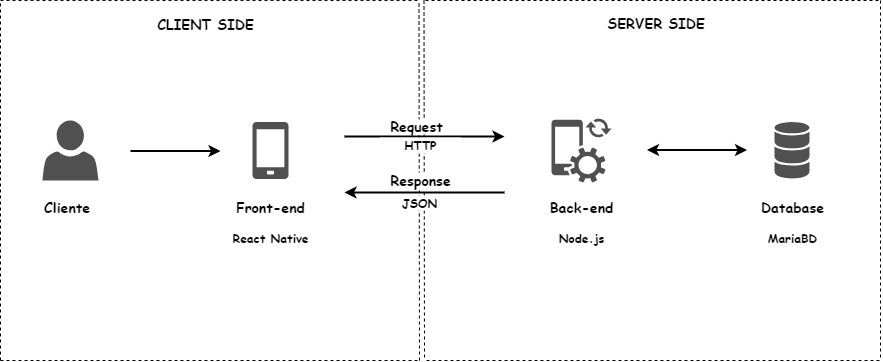
\includegraphics[width=15cm]{ArquiteturaSoftware.png}\\
    \caption{“Diagrama de Arquitetura de Software”}
        Fonte: Os autores
    \label{fig:infografico}
\end{figure}

    Essas tecnologias foram selecionadas para proporcionar uma experiência de usuário fluida e escalável, alinhada às necessidades específicas da aplicação Voz Feminina, visando proporcionar uma experiência de usuário otimizada, com desempenho elevado e manutenção simplificada.
    
\bibliography{referencias}

\end{document}